%
% chapter3.tex
%

\chapter{NVIDIA Bluefield-3}
\label{cha:design}
Die im Rahmen dieser Arbeit verwendete SmartNIC ist die von Nvidia im Jahre 2022 veröffentlichte Bluefield-3. Wie bereits am Namen der Karte zu erkennen ist, handelt es sich dabei um die dritte Generation von Netzwerkkarten, die zusätzlich zur netzwerkspezifischen Architektur noch einen allgemeinen ARM-Prozessor verbaut hat. Zusätzlich wird in einem späteren Abschnitt ein Überblick über das DOCA-Framework gegeben, welches von NVidia als einheitliche Programmierschnittstelle veröffentlicht wurde, um die Programmierung der Hardware von der jeweiligen Generation unabhängig zu machen.
\section{Entstehung}
Die Entwicklung der BlueField ist ein Produkt der letzten Dekade, in der ein immerwährend größeres Interesse an der Effizienzsteigerung von Rechenzentren entstanden ist. Energiesparende Systeme, die dieselbe Leistung erreichen wie selbige Integration auf einem allgemeinen Prozessor, bieten für Systemintegratoren eine ausgezeichnete Möglichkeit, auch vor dem Hintergrund des Klimawandels energieoptimierte Systeme zu entwickeln.
\subsection{BlueField-1}
Die erste Generation der Bluefield-Hardware (siehe Abbildung 4.1) wurde im Jahre 2017 von Mellanox Technologies vorgestellt und bildet den ersten Eintrag in die Reihe der Bluefield-SmartNIC-Serie. Sie kombinierte erstmalig die ConnectX-5-Plattform mit einem ARM-basierten System-on-Chip. Die Idee dahinter war es, das Verhalten der Netzwerkplattform mittels User-Anwendungen beeinflussen zu können. Dazu wurde eine API zwischen der ConnectX und dem ARM-Prozessor entwickelt. Hierzu sei erwähnt, dass es sich bei der ConnectX-Plattform um eine bereits weit verbreitete und in viele Systeme integrierte Hardware handelte. Sie besaß bereits zum damaligen Zeitpunkt eine breite Anzahl von paketbasierten Operationen, mit deren Hilfe eine weitreichende Manipulation sowie Paket-Steering oder anderweitige Verwendungen ermöglicht wurden. Die BlueField-1 war mit einem ARM-A72 mit 4 Kernen und 8 Threads ausgestattet und besaß außerdem zwei QSFP28-Anschlüsse, welche bis zu 100 Gbps Durchsatz erreichen konnten. Die Zielgruppe der BlueField-Serie waren von Anfang an der Enterprise-Markt sowie die zahlreichen größeren Rechenzentren, in denen Rechenoperationen ausgeführt werden, die auf mehreren Computern eines Clusters oder einer Clusterstruktur ausgeführt werden. Gerade in diesem Umfeld wird eine derartige Architektur von Interesse, da der Netzwerkverkehr so anwendungsspezifischer verteilt werden und somit die Effizienz eines Rechnerverbundes steigern kann. \cite{bluefieldhistory}
\begin{figure}
    \centering
    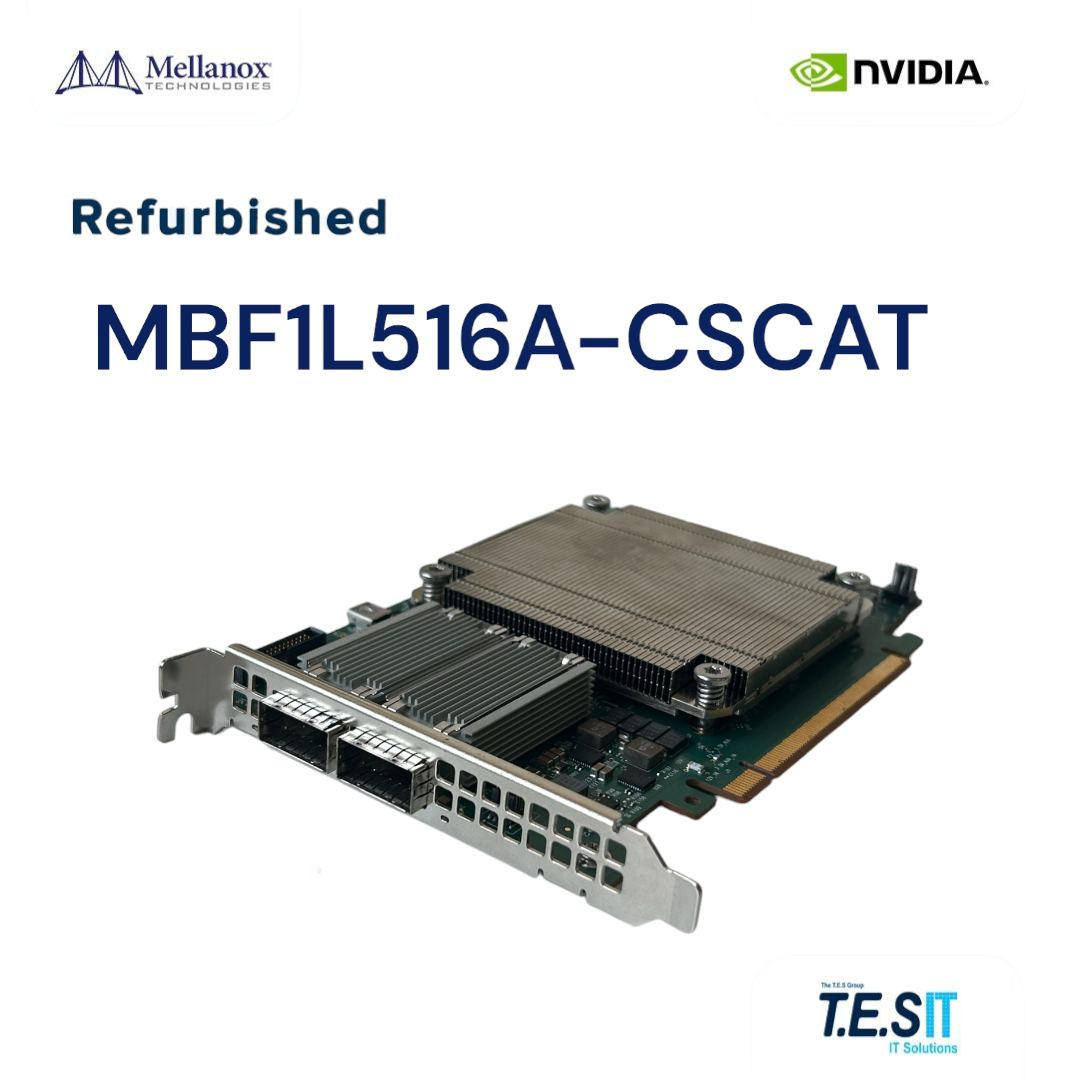
\includegraphics[width=0.65\linewidth]{images/s-l1600.png}
    \caption{BlueField-1-Karte \cite{ebay_bluefield1_2025}}
    \label{fig:enter-label}
\end{figure}
\subsection{BlueField-2}
Nach der Übernahme von Mellanox durch den Chip-Hersteller NVIDIA im Jahre 2019 wurde das Projekt BlueField von NVIDIA nicht nur weitergeführt, sondern mit dem Aufkommen von vermehrten Machine Learning Workloads sogar das Marketing ausgebaut. So wurde die BlueField-2 im Jahre 2021 unter dem neuen Hersteller NVIDIA veröffentlicht und bot nun einen QSFP56, der laut eigenem Marketing-Material bis zu 200 Gbps erreichen sollte. Abermals kam der ARM-A72 zum Einsatz, der erneut mit 4 Kernen und 8 Threads verbaut wurde. \cite{bluefieldhistory} Erstmalig wurde außerdem damit geworben, dass ein Einsatz in Machine-Learning-Rechenclustern besonders wertvoll sei. Auf Angaben, warum genau das der Fall sein sollte, wurde seitens des Herstellers verzichtet. Insbesondere nicht vor dem Hintergrund, warum es sich dabei nun um ein Alleinstellungsmerkmal anderen SmartNICs gegenüber handeln sollte.
\subsection{BlueField-3}
Zuletzt wurde im Jahre 2022 die BlueField-3 veröffentlicht, die im Rahmen dieser Arbeit zur Verwendung kam. Erstmalig wurde nun der ARM-A78 mit 8 Kernen und somit 16 Threads verbaut. Die Arbeitsspeicherarchitektur nahm zusätzlich auch den Generationensprung von DDR4 auf DDR5 vor und verwendet so einen deutlich schnelleren Speichertakt als die vorherige Generation. Außerdem wurde erneut der Netzwerkanschluss aktualisiert und verwendet nun den QSFP112. Laut NVIDIA soll mit diesem Netzwerkverbund eine Line Rate von bis zu 400 Gbps erreicht werden. \cite{battle} Dabei wird im Marketing-Material nicht explizit erwähnt, welche Paketgröße für besagten Durchsatz verwendet wurde. Erneut soll laut NVIDIA der Fokus der Hardware vermehrt auf dem Einsatz in Rechenzentren liegen, in denen größere Machine-Learning-Lasten laufen. Die BlueField-3 soll daraufhin die Rolle einer intelligenteren Paketverteilung einnehmen, wobei die Last der Lastverteilung nicht mehr auf dem Hostsystem bzw. dem entsprechenden Host-Prozessor liegt, sondern eben auf der Netzwerkkarte selbst. Außerdem sind eine Menge von weiteren speziellen hardwarebeschleunigten Hardwareeinheiten auf der neuesten Iteration der BlueField-Serie verbaut worden. Alle genannten Generationen BlueField werden per PCI-E-Stecker in den Hostsystemen verbaut und verwenden so den aktuellsten PCI-E 5.0 Standard, der auf eine theoretische Maximalbandbreite von 32 Giga Transfer/s kommt. Somit soll eine ultraschnelle Schnittstelle zwischen Hostsystem und BlueField-3 erreicht werden (siehe Abbildung 4.2).
\section{Architektur}
Um der Funktion einer intelligenten Netzwerkkarte nachzukommen, sind auf der BlueField diverse Hardwareeinheiten verbaut, die eine Reihe von Einsatzzwecken abdecken sollen. Dabei werden nicht alle angebotenen Funktionen auch tatsächlich von ASIC-Hardwareeinheiten übernommen, sondern werden teilweise komplett oder nur in bestimmten Pipelineabschnitten auf dem ARM-Core ausgelagert, um dort einer weiteren Behandlung unterzogen zu werden. Wie in Abbildung 3.2 zu erkennen ist, gliedert NVIDIA die BlueField-Karte grob in Domänen unterschiedlichster Funktion auf. Abgesehen vom ARM-Teil der Karte, womit im Wesentlichen der Bereich beschrieben wird, in dem der Prozessor, Arbeitsspeicher und restlicher I/O zusammengefasst werden, sind die beiden Bereiche \textbf{Accelerators} und \textbf{Accelerated Programmable Pipeline} diejenigen, in denen eine große Menge der eigentlichen Hardwarebeschleuniger sitzen. Allerdings geht aus dem von NVIDIA bereitgestellten Material nicht vollständig hervor, worum es sich bei dem sogenannten Datapath Accelerator handelt. \cite{nvidia_bluefield_dpu}  Im Release-Flyer der BlueField-3 steht allerdings, dass es sich dabei auch um einen Prozessor mit 16 Kernen handeln soll, der mit 256 Threads ausgestattet ist. Dies würde bedeuten, dass jeder Kern von Hause aus 16 Threads besitzt. Zusätzlich wird oft darauf verwiesen, wie einfach ein Zusammenspiel von DPU und Hostsystem mittels der PCI-E-Anbindung funktionieren soll. Im Folgenden wird eine Auswahl aus Beschleunigern und Funktionen vorgestellt, die vom Hersteller  angeboten werden. \cite{nvidia_bluefield_dpu} 
\begin{figure}
    \centering
    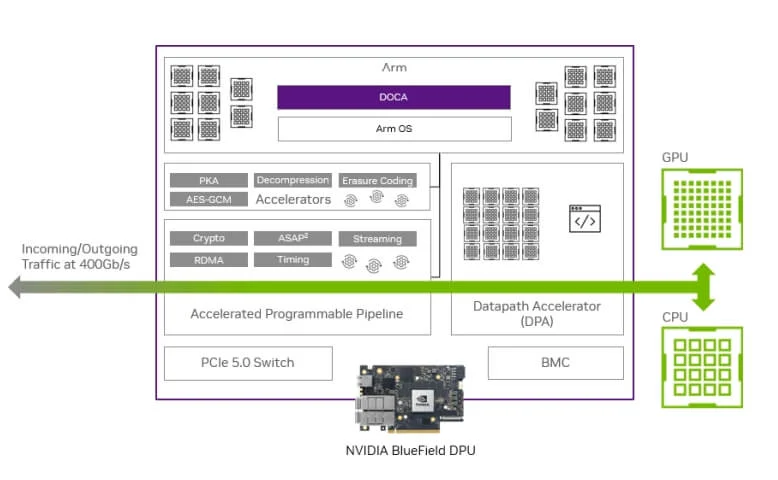
\includegraphics[width=1\linewidth]{images/nvda-bluefield-dpu.png}
    \caption{BlueField-3 Architektur}
    \label{fig:enter-label}
\end{figure}
\subsection{Hardwareeinheiten}
Im Folgenden wird eine Auswahl von Hardwarebeschleunigern vorgestellt.
\subsubsection{PKA}
PKA steht für Public-Key-Acceleration und bietet eine Reihe von Funktionalitäten im Zusammenhang mit der Arbeit mit öffentlichen Schlüsseln im Kontext von SSL-Anwendungs-fällen. So stellt es beispielsweise einfache bis komplexere arithmetische Operationen wie RSA, Diffie-Hellman sowie Addition und Subtraktion bereit. Es soll eine einfache Programmierschnittstelle bieten, sobald die DOCA-Applikation mit Verschlüsselungen hantiert, die möglichst schnell umgesetzt werden sollen.
\subsubsection{Decompression}
Die Dekompressionsbeschleuniger der BlueField-3 sollen vor allem dann zum Tragen kommen, wenn die Netzwerkkarte mit Buffern konfrontiert wird, in denen die Daten komprimiert vorliegen. Dabei soll sich diese möglichst nicht auf die Verarbeitung des Datenverkehrs auswirken.
\subsubsection{Erasure Coding}
Erasure Coding bezeichnet die Hardwareeinheit, deren hauptsächliche Funktion die Forward Error Correction ist. Dies wird dazu verwendet, um eventuelle Übertragungsfehler oder umgedrehte Bits mithilfe der Paritätsinformation reparieren zu können.
\subsubsection{AES-GCM}
Advanced-Encryption-Standard (AES) ist ein bekannter Verschlüsselungsstandard, der quasi von jedem Endgerät dieser Welt implementiert wird, um modernen Sicherheitsanforderungen gerecht zu werden. Hierzu hat NVidia eine Hardwareeinheit entwickelt, um Daten auch im eigenen Arbeitsspeicher verschlüsseln zu können.
\subsubsection{RDMA}
RDMA ist die Abkürzung für Remote Direct Memory Access. Innerhalb eines solchen Prozesses kann ein Prozess auf den Speicherbereich eines anderen Rechners zugreifen. Damit wird eine Alternative zum klassischen Netzwerkverkehr angeboten.
\subsection{Datapath Accelerator}
Der Datapath Accelerator, kurz DPA, ist für diese Arbeit von besonderem Interesse, da laut NVidia hier ein Großteil der Netzwerkverarbeitung vorgenommen wird. Wie bereits im vorherigen Kapitel zum Hardwareaufbau erwähnt, soll hier ein weiterer Prozessor zum Einsatz kommen, der über ein extremes 16-faches Multithreading verfügt. Dieses Multithreading wird benötigt, um möglichst latenzfreie Verarbeitung umzusetzen. \cite{nvidia_dpa_subsystem_2025} Leider sind seitens des Herstellers allerdings keine weiteren Angaben zur verbauten Hardware freigegeben worden. Daher ist es ohne weitere Informationen nicht möglich, die genauere Funktionsweise zu analysieren. Dennoch sollte es, sofern es sich dabei denn wirklich um den trafficverarbeitenden Prozessor handelt, in den späteren Messungen zu beobachten sein, dass der ARM-Prozessor von dem eingehenden Verkehr unberührt bleiben sollte.

\section{DOCA Framework}
DOCA ist ein von NVidia entwickeltes Framework, das speziell für die BlueField-Karten entwickelt wurde. Es gliedert sich in verschiedene Teilbereiche und unterscheidet dabei zwischen architektonischen Grundsätzen, Programmierinterfaces, aber auch dem Betriebssystem für die Karte selbst. Allgemein ist DOCA dafür gedacht, der direkte Anlaufpunkt für Entwickler zu sein, die auf der BlueField-Plattform entwickeln wollen. Damit werden auch Dinge wie Programmiersprachen, Programmierparadigmen und eine Reihe von bereits angelegten Bibliotheken bereitgestellt. Zusätzlich werden sämtliche Hardware-Treiber ebenfalls unter dem Oberbegriff DOCA zusammengefasst. \cite{nvidia_doca_framework} Im Folgenden wird ein Überblick zu DOCA im Allgemeinen gegeben und ein besonderes Augenmerk auf die für diese Arbeit relevanten Teilbereiche gelegt  (siehe Abbildung 4.3).
\begin{figure}
    \centering
    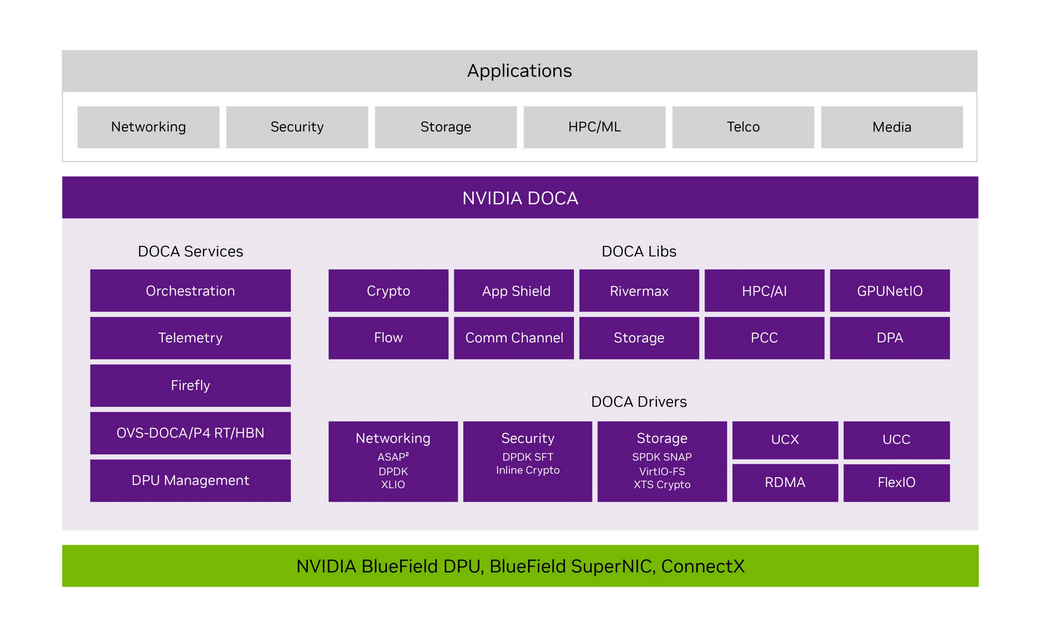
\includegraphics[width=1\linewidth]{images/Screenshot 2025-04-26 at 08-31-41 DOCA Overview - NVIDIA Docs.png}
    \caption{Überblick der Teilbereich von DOCA}
    \label{fig:enter-label}
\end{figure}
\subsection{DOCA Services}
DOCA stellt eine Reihe von Services bereit, die vorrangig dazu dienen sollen, eine Ende-zu-Ende-Lösung für einen speziellen Anwendungsfall zu bieten. Dazu gliedert NVidia diverse (Abbildung 3.3) Unterkategorien aus. Einerseits aufgrund des primären Anwendungsfeldes in Rechenzentren wird viel Wert auf Orchestrierung gelegt. Leider bleibt NVidia hier bemerkenswert ungenau, was genau damit eigentlich gemeint ist. Bei der Telemetrie hingegen stellt NVidia eine große Schnittstelle bereit, um genaue hardwarebezogene Daten abrufen zu können. Hierzu werden den Entwickelnden zwei Tools bereitgestellt. Das Tool \textbf{doca\_telemetry\_diag} stellt die Konfiguration des Loggings dar. Dazu kann mithilfe besagter Tools festgelegt werden, welche Telemetriedaten und auch in welchem Samplingintervall erhoben werden sollen. Diese Daten können dann in diversen auswählbaren Dateiformaten abgerufen werden. \textbf{doca\_telemtery\_pcc} soll den Zugang zu speziellen algorithmischen Daten ermöglichen. Damit sind die bereits in DOCA vorimplementierten Funktionen gemeint, die meist hardwarebeschleunigt, also außerhalb des sichtbaren Bereichs des ARM-Hosts, ausgeführt werden. Sonstige Services wie beispielsweise der Firefly sind NVidias Implementierungen des Precision Time Protocols. Ziel dieses Protokolls ist es, die Zeit innerhalb eines Clusters möglichst genau propagieren zu können. Dazu verspricht NVidia, möglichst viel von dieser Komplexität vor dem Anwender mithilfe von Firefly fernzuhalten. Außerdem setzt NVidia zur Konfiguration des Datenverkehrs stark auf die Integration von Open vSwitch (OVS). Dazu wurde eigens ein eigener Service entwickelt, der abermals die eigentliche Komplexität des Konfigurationsprozesses dem Entwickler abgenommen werden soll. Hauptgrund ist allerdings vermutlich, dass, um mit den spezifischen Hardwareeinheiten überhaupt kommunizieren zu können, die Open vSwitch-Interfaces angepasst werden müssen. 
\subsection{DOCA Bibliotheken}
Damit eine reibungslose Inbetriebnahme sowie Programmierung einer SmartNIC erfolgen kann, muss klar definiert sein, wie, sofern programmatische Konfigurationen erfolgen sollen, ein Entwickler mit der entsprechenden Hardwareeinheit kommunizieren kann. Damit ist es nicht mehr nötig, die Feinheiten der einzelnen Hardwarekommunikationskanäle zu implementieren, sondern es kann auf eine mehr oder weniger vereinheitlichte Programmierschnittstelle zugegriffen werden. Dazu stellt NVidia Programmbibliotheken in Form von C-Headern bereit, mithilfe derer intrinsische Funktionen auf der Architektur ausgeführt werden können. Dabei lässt sich grob formulieren, dass jede in Kapitel 3.2.1 genannte Hardwareeinheit eben auch eine entsprechende Bibliothek bekommen hat. Zusätzlich gibt es aber auch Bibliotheken, die Funktionen wie Speicherverarbeitung für Anwendungsfälle wie verteilte Speichersysteme implementieren.
\subsection{DOCA Flow}
DOCA Flow ist die Bibliothek, die die Verarbeitung und Modifikation von Netzwerkpaketen enthält. Das Versprechen seitens NVidia ist hierbei, dass alle Funktionen von Flow auf den Hardwarebeschleunigern ausgeführt werden können. DOCA Flow wird, wie viele moderne Systeme, deklarativ programmiert. Das bedeutet, der State des aktuellen Netzwerkverkehrs ist immer genau so, wie er durch die Konfiguration deklariert wurde. Dies hat den großen Vorteil, dass die Entwicklung und in der Folge auch das Debugging sich immer direkt mit dem Programmcode selbst befassen kann, da keine Fehler zur Laufzeit entstehen können (sollten) die so nicht klar vorher definiert worden sind.
Allgemein ist DOCA Flow darauf ausgelegt, statt Pakete einzeln zu behandeln, in Netzwerkdatenpfaden den Verkehr zu steuern. Dazu werden die Hardwareregeln wie beispielsweise \textbf{Packet Matching}, \textbf{Forwarding} und \textbf{Monitoring} definiert. Beim Packet Matching wird ein Zusammenspiel aus Filter- und Match-Regeln verwendet, um Pakete aus dem Datenfluss der NIC auszuwählen und der entsprechenden Pipe zuzuordnen (siehe Abbildung 4.4). \cite{nvidia_doca_flow_2025}
\subsubsection{Flow Pipe}
\begin{figure}
    \centering
    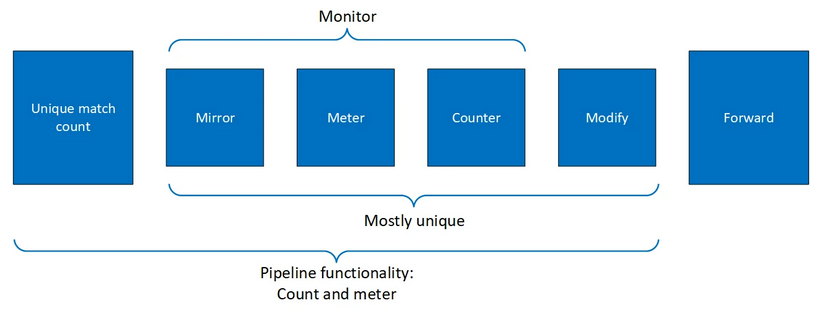
\includegraphics[width=1\linewidth]{images/pipe.png}
    \caption{Schemata und Zugehörigkeiten einer Flow Pipe}
    \label{fig:enter-label}
\end{figure}
Eine Flow Pipe beschreibt einen genannten Datenpfad, der deklarativ an die BlueField-3 API übergeben wird. Dabei setzt sich eine Flow Pipe immer aus den vier wesentlichen Bestandteilen \textbf{Match}, \textbf{Monitor}, \textbf{Action} und \textbf{Forward} zusammen. Diese Bestandteile können in \textbf{Entries} organisiert werden. Sie bilden die tatsächlichen aktiven Teile der Pipe. Pipes bilden eine Abstraktion eines Datenpfades, auf denen die einzelnen Entries angewendet werden.

Beim Match wird mithilfe einer Zusammensetzung aus Filtern und Match-Regeln klar definiert, welche Pakete aus dem Datenstrom der BlueField genommen werden sollen und welcher entsprechenden Pipe zugeordnet werden. 

Daraufhin wird das Paket laut Dokumentation gespiegelt und dem Monitorteil übergeben. Dieser erlaubt es, Daten über die Pipe auszulesen. So kann zur Laufzeit die Anzahl der von der Pipe verarbeiteten Pakete sowie deren Größe in Bytes ausgelesen werden. Im Verlauf der Messung im späteren Teil wurde der Versuch durchgeführt, ob ein ein- bzw. ausgeschaltetes Monitoring Auswirkungen auf die Leistungsfähigkeit der Karte hat. Dies ist klar zu verneinen. Weder Bandbreite noch Pakete/Sekunde wurden von dem Monitoring beeinflusst.

Nachdem nun Pakete in der entsprechenden Flow Pipe ankommen, können nun eine Reihe von Aktionen auf diese ausgeführt werden. Diese Funktionen werden in Entries durchgeführt. Darunter befinden sich vor allem Funktionen, die die Ethernet- sowie IP-Header modifizieren können. Es ist so beispielsweise nicht ohne weiteres möglich, Pakete einzeln zu verarbeiten, sondern nur Klassen von Paketen, die eben in der entsprechenden Pipe bzw. dem entsprechenden Entry angekommen sind. Die eigentliche Payload des Paketes kann \textbf{nicht} von Flow verarbeitet werden. Dies ist vor allem der Tatsache geschuldet, dass es sich hierbei eben um die Programmierung von Hardwarebeschleunigern handelt. Würden wir Pakete einzeln verarbeiten wollen, so müssten diese zur Laufzeit auf den Prozessor der SmartNIC gebracht werden, was mit erheblichen Leistungseinbußen einhergehen würde.
Die Payload der Pakete kann nicht verarbeitet werden, da diese eine variable Länge besitzen kann, was ein Problem für eine feste Hardwarearchitektur darstellt. Bei festgelegten Header-Bitfeldern allerdings kann eine festdefinierte ASIC-Hardware gut die entsprechenden Bits mithilfe von einfachen logischen Bauteilen verarbeiten (siehe Abbildung 4.5).  \cite{nvidia_doca_flow_v1_2} 
\begin{figure}
    \centering
    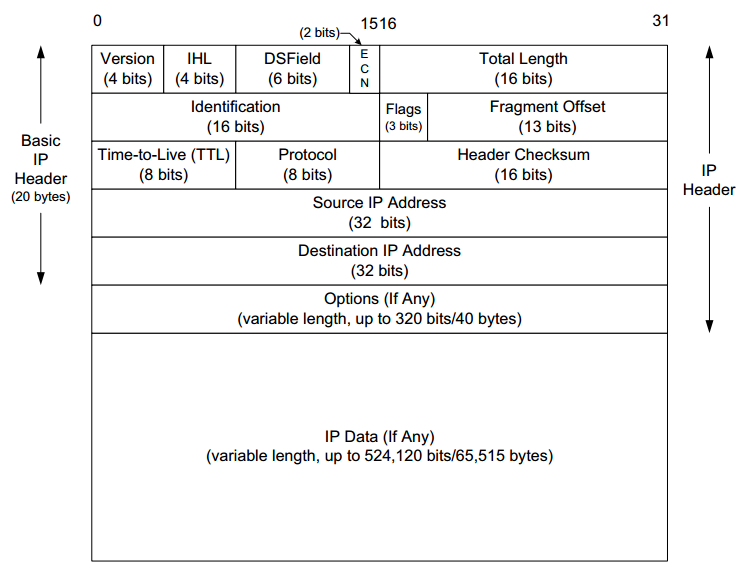
\includegraphics[width=0.8\linewidth]{images/figure_5-1.png}
    \caption{Aufbau eines IP-Headers}
    \label{fig:enter-label}
\end{figure}
In Abbildung 4.5 ist zu erkennen, dass sich bestimmte Teile eines Headers immer an genau der gleichen Stelle im Bitfeld befinden. So muss die Hardware nicht erst parsen bzw. erkennen, wo im Paket sich welche Daten befinden.

Zuletzt kann in einer Pipe aber auch in den Entries selbst mittels des \textbf{Forward} festgelegt werden, wohin die relevanten Pakete geleitet werden sollen. Dabei kann sowohl direkt auf einen Port, der einem entsprechenden Hardware-Port auf der Karte gleicht, eine andere Pipe oder gar kein Folgeziel gewählt werden. Bei letzterem handelt es sich logisch um einen Drop des Pakets. Von besonderem Interesse ist allerdings die Funktion, in eine andere Pipe weiterzuleiten, da sich so komplexere Anwendungen umsetzen lassen, in denen einzelne Pipes bestimmten Traffic verarbeiten und mehrere Datenströme modifiziert werden können. Allgemein bietet DOCA Flow die Kategorisierung dieser Pipes. Dabei wird zwischen sogenannten \textbf{Steering Domains} unterschieden. Diese verbieten gewissen Pipefunktionen, wenn der entsprechenden Domain eine Pipe hinzugefügt wurde. 
\begin{figure}
    \centering
    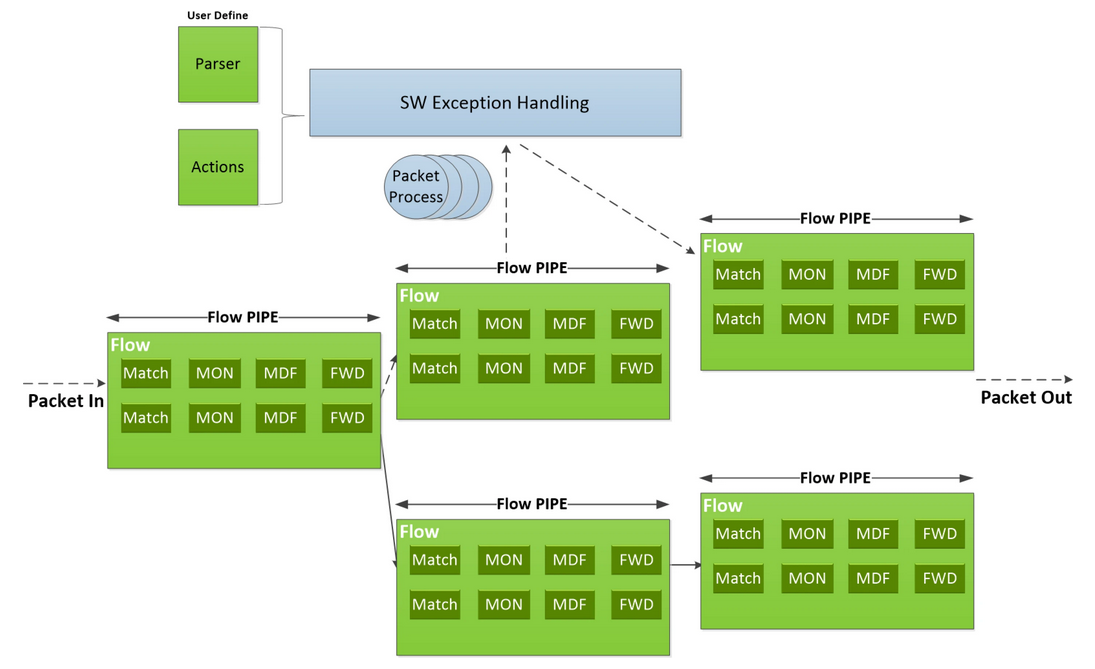
\includegraphics[width=1\linewidth]{images/Screenshot 2025-04-30 at 11-16-05 DOCA Flow - NVIDIA Docs.png}
    \caption{Beispielhafter Flow-Pipe-Aufbau}
    \label{fig:enter-label}
\end{figure}

In Abbildung 4.6 ist eine Beispielanwendung per Diagramm zu sehen, in der eine Verkettung von Flow Pipes erfolgt ist. Es ist auch möglich, dass, wenn Pakete nicht von einer entsprechenden Pipe gefangen werden, sie an einen Hostkern durchgereicht werden. Dort kann dann ein weiteres Programm laufen, welches daraufhin diese Pakete verarbeitet. Dabei verlässt das Paket allerdings den hardwarebeschleunigten Bereich und ist wieder an die Performance des ARM-Cores gebunden.
\subsubsection{Flow Entry}
\begin{figure}
    \centering
    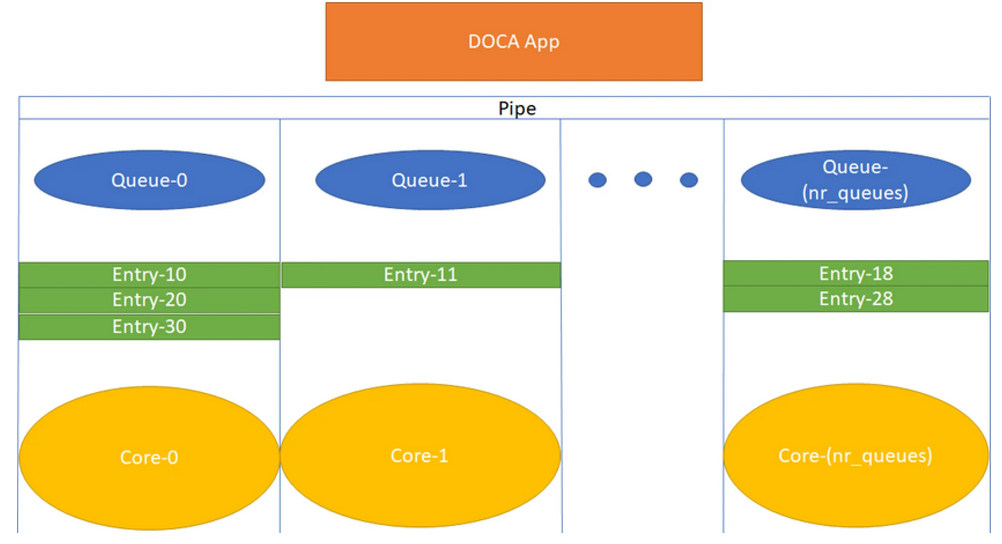
\includegraphics[width=1\linewidth]{images/entries.png}
    \caption{Auslagerung von Pipe Entries}
    \label{fig:enter-label}
\end{figure}
Laut NVidia werden Entries einer Flow Pipe auf mehreren Kernen des Data Accelerators verarbeitet. Jedem dieser Kerne ist eine entsprechende Queue mit den zu verarbeitenden Paketen zugeordnet  (siehe Abbildung 4.7). Durch diese Parallelisierung soll es möglich sein, dass der Paketverkehr ohne Latenzzugewinn verarbeitet werden kann. Leider waren im Rahmen dieser Arbeit keine weiteren Daten, wie genau diese Lastverteilung auf den 256 Threads funktioniert, auffindbar. Flow Entries können spezielle Aufgaben für eine Pipe übernehmen. So werden beispielsweise in XenoFlow die Entries genutzt, um pro Entry an ein bestimmtes Backend weiterzuleiten. Entries sind allerdings lose an die Pipe-Definitionen gebunden. Soll beispielsweise in einem Entry entschieden werden, ob an Port 0 oder Port 1 weitergeleitet werden soll, so muss in der Pipe das entsprechende Forward-Feld auf 0xffff gesetzt sein, damit die Hardware weiß, dass der Forwardschritt erst im Entry erfolgt. Selbiges gilt natürlich für Matching und Actions.
\subsubsection{Packet Matching}
Für die Funktion eines Lastverteilers ist eine der Hauptfunktionen, den gesamten Traffic in handhabbarere Teillasten zu modulieren, damit diese dann auf verschiedene Backends verteilt werden können. Dazu ist eine Art des Packet Matchings besonders praktisch. 
\begin{figure}
    \centering
    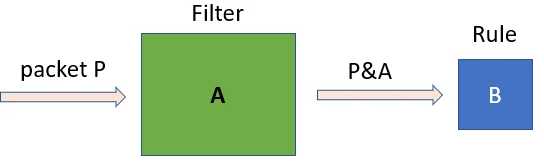
\includegraphics[width=1\linewidth]{images/paketmatchng.png}
    \caption{Matching Schema der BlueField}
    \label{fig:enter-label}
\end{figure}
Das Packet-Matching aus DOCA Flow ist in Abbildung 4.8 zu sehen. Zunächst erreicht ein Paket den Filter und wird mit diesem auf der Bit-Ebene verundet. Sprich, das Ausgabebitfeld besitzt an einer Position eine 1, wenn das Datenpaket und der Filter an der gegebenen Stelle auch eine 1 gesetzt haben. So kann eine Art Vorauswahl realisiert werden, in der Entwickler festlegen können, welche Bits des entsprechenden Feldes überhaupt analysiert werden sollen. Daraufhin erreicht das neu berechnete Bitfeld die Regel. In dieser wird überprüft, ob das Bitfeld der Regel entspricht. Wenn dies der Fall ist, so wird das Paket dem Match zugeordnet. Wird die Regel nicht erfüllt, wird das Paket fortan als Miss betrachtet.
\begin{itemize}
  \item Sei $P \in \{0,1\}^n$ das eingehende Paket als Bitfeld.
  \item Sei $F \in \{0,1\}^n$ das Bitfeld gibt als Maske an welche Bits berücksichtigt werden sollen
  \item Die bitweise Filterung erfolgt durch eine Konjunktion  
  \[
    P_{neu} = P \land F = (P_1 \land F_1, P_2 \land F_2, \dots, P_n \land F_n)
  \]
  \item Sei $R \in \{0,1\}^n$ das Bitmuster der Rule. Ein Paket wird als \emph{Match} klassifiziert, wenn gilt:
  \[
    P_{neu} = R
  \]
  \item Sonst wird das Paket als \emph{Miss} behandelt:
  \[
    P_{neu} \ne R
  \]
\end{itemize}

In der Matching-Deklaration kann außerdem unterschieden werden, ob Pakete explizit oder implizit gematcht werden sollen. Damit kann festgelegt werden, ob wir wie beim expliziten Match das genaue Bitfeld aus dem Datenfluss extrahieren wollen. Alternativ können wir mittels des impliziten Matchens Muster aus den Bitfeldern extrahieren. Sogleich können mehrere Bitfelder extrahiert werden, sofern diese die deklarierten Muster enthalten.


Sobald Bitfelder allgemein verarbeitet werden sollen, so muss dies mithilfe eines C Structs klar definiert werden. Dazu werden alle Bits des gewünschten Bitfeldes beim Definieren der Datenstruktur zunächst auf 1 gesetzt.
In XenoFlow sieht eine Filter-Implementierung, die alle IP-Adressen in Gerade- und Ungerade-Klassen teilt, wie folgt aus:
\begin{minted}{c}
match.outer.ip4.src_ip = BE_IPV4_ADDR(255, 255, 255, 255);
match_mask.outer.ip4.src_ip = BE_IPV4_ADDR(0, 0, 0, 1);
\end{minted}
Somit ist die Match-Maske aktiviert. Dies bedeutet, dass wir nun nicht auf exakte Bitfelder matchen, sondern mittels der Match-Maske Bitmuster deklarieren können, die wir dann in den Entries matchen können. Das bedeutet, nur allein die Match-Maske in der Pipe führt noch nicht zu Paketen, die gematcht werden. Es bedarf in der gezeigten Konfiguration immer noch eines speziellen Matches im Entry wie folgt: 
\begin{minted}{c}
match.outer.ip4.src_ip = BE_IPV4_ADDR(0, 0, 0, 1);
\end{minted}
Die Kombination aus Pipe-Match und Entry-Match würde nun alle Pakete dem Entry zuordnen, die eine IP-Adresse haben, deren Quell-IP am letzten Bit eine 1 gesetzt hat.
\subsection{DOCA Treiber}
Damit die entsprechenden Hardwareeinheiten vom ARM-SmartNIC-System aus betrieben werden können, hat NVidia eigens bestimmte Treiber entwickelt. Dazu zählt unter anderem auch eine DPDK-Implementierung. DPDK steht für Data Plane Development Kit und ist ein von der Linux Foundation verwaltetes Open Source Projekt. Es wird verwendet, um Kernelprozesse der Datenverarbeitung aus dem Linuxkernel in den Userspace zu verlagern, um dort eine Verarbeitung vorzunehmen. DOCA Flow nutzt somit DPDK, um die Pakete von dem Data Accelerator auf den ARM-Kern in den Userspace zu bringen, da DOCA Applikationen im Userspace ausgeführt werden. 

Außerdem hat NVidia in DOCA andere Treiber entwickelt, wie beispielsweise Virtio-FS, mithilfe derer eine kompakte Integration von Dateisystemen in die BlueField-Systeme vorgenommen werden kann. Ein denkbarer Einsatzzweck wäre die dynamische Anbindung von Persistent Volumes in einem Kubernetes-Cluster, sofern sich die Volumes auf einem anderen Knoten befinden als der Pod, der versucht, das entsprechende Persistent Volume zu claimen.
\subsection{Anwendungen}
DOCA stellt eine Reihe von bereits implementierten Applikationen bereit, die eine Reihe von denkbaren Anwendungszwecken von DOCA präsentieren sollen. Im Rahmen dieser Arbeit wurden drei dieser Applikationen näher betrachtet.

\textit{So ist in einem Flyer auch von einem Load Balancer die Rede. Allerdings war dieser nicht auffindbar.}

\subsubsection{Firewall}
Hier hat NVidia eine beispielhafte Firewall-Applikation entwickelt, deren Sinn und Zweck es ist, mit Hilfe von gRPCs zwischen Host und SmartNIC dynamisch Hardwareregeln hinzuzufügen bzw. diese wieder zu entfernen. Dabei wird der Host von dieser Aufgabe entlastet und die Pakete werden nicht erst auf dem Zielsystem, sondern bereits auf deren Netzwerkkarten verworfen.

\subsubsection{GPU Packet Processing}
Sollte im Hostsystem zusätzlich zur BlueField auch noch eine GPU verbaut sein, so bietet DOCA eine Applikation an, mit deren Hilfe Pakete von der GPU verarbeitet werden können. Das könnte beispielsweise für Anwendungen sehr nützlich sein, in denen nicht nur Header-Bitfelder verarbeitet werden, sondern auch die Payloads der Pakete verarbeitet werden sollen. Dazu eignen sich die Vektoreinheiten einer Grafikkarte gut, da diese auf hochdimensionale Vektorräume ausgelegt sind. 

\subsubsection{Switch}
Die Kommunikation zwischen Host-System und der DPU wird mittels verschiedener Hardware-Networking-Interfaces angeboten. Bei der Switch-Applikation wird der Netzwerkverkehr auf der DPU in verschiedene Teilverkehre gespaltet und dann auf mehrere dieser Networking-Interfaces weitergegeben. Dadurch wird abermals das Hostsystem entlastet, da die spezielle Fallunterscheidung eines jeden Pakets nicht mehr vom Prozessor des Hosts übernommen werden muss, sondern bereits auf der Netzwerkkarte passiert. Außerdem bietet die SmartNIC-Architektur zusätzlich die Möglichkeit, bestimmte Hardwarebeschleuniger für diesen Einsatzzweck zu verwenden.